\documentclass[11pt,a4paper]{article}
\usepackage[margin=18mm,top=22mm,bottom=20mm]{geometry}
\usepackage{fontspec}\setmainfont{Latin Modern Roman}
\usepackage{xcolor}\usepackage{amsmath,amssymb,tikz,graphicx,fancyhdr,array,needspace}
\usetikzlibrary{patterns,arrows.meta,decorations.pathmorphing,calc}
\setlength{\headheight}{14pt}
\usetikzlibrary{arrows.meta}
\pagestyle{fancy}\fancyhf{}\renewcommand{\headrulewidth}{0.4pt}
\fancyhead[L]{\textbf{M-05}}\fancyhead[C]{\itshape Fizika — yechimlar (OliyFizika.uz)}\fancyhead[R]{\textbf{Mock №5}}
\fancyfoot[C]{\thepage}
\setlength{\parindent}{0pt}\setlength{\parskip}{3pt}
\newcommand{\opt}[2]{\hspace*{4mm}#1)\ #2\par}
\newcommand{\blank}{\rule{5cm}{0.4pt}}
\begin{document}

\begin{center}{\Large\textbf{FIZIKA — YECHIMLAR}}\\[2pt]{\large Mock №5}\end{center}
\Needspace{10\baselineskip}\noindent\begin{minipage}{\linewidth}
\textbf{1.}\ Blokni kötarib turgan ipning taranglik kuçi 36 N bölsa, blokka ilingan yukning oğirligi (N) aniqlansin. (blok vaznini inobatga olmang)\par\smallskip
\noindent\hspace*{4mm}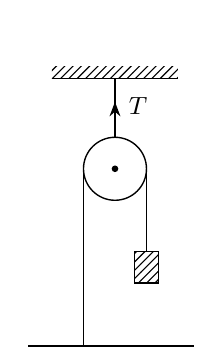
\begin{tikzpicture}[x=1cm,y=1cm,line width=0.5pt,>=Stealth,font=\small]
\fill[pattern=north east lines,draw=none] (0,3.4) rectangle (1.6,3.55); \draw (0,3.4)--(1.6,3.4);
\draw (0.8,3.4)--(0.8,2.65); \node[right] at (0.85,3.05) {$T$}; \draw[->] (0.8,3.0)--(0.8,3.1);
\draw[fill=white] (0.8,2.25) circle(0.4); \fill (0.8,2.25) circle(1.2pt);
\draw (0.4,2.25)--(0.4,0.0); \draw (1.2,2.25)--(1.2,1.2);
\draw[pattern=north east lines] (1.05,0.8) rectangle (1.35,1.2);
\draw (-0.3,0)--(1.8,0); \fill[pattern=north east lines,draw=none] (-0.3,-0.15) rectangle (1.8,0);
\end{tikzpicture}\par\smallskip
\opt{A}{36}
\opt{B}{72}
\opt{C}{9}
\opt{D}{18}
\end{minipage}\vspace{2pt}\par
\noindent\colorbox{gray!12}{\parbox{\dimexpr\linewidth-2\fboxsep}{\textbf{Javob: D) 18}}}\par\smallskip
\noindent\textit{Yechim.}\ Blok orqali ötgan ipning bir uçi polga mahkamlangan, ikkinçisiga yuk ilingan. Ip böylab taranglik bir xil va yuk muvozanatda bölgani uçun $T_{ip}=P$. Vaznsiz blokning muvozanati: $T=2T_{ip}$, bundan $P=T/2=18$ N.\par\par\medskip\hrule\medskip
\Needspace{10\baselineskip}\noindent\begin{minipage}{\linewidth}
\textbf{2.}\ Massasi 3 kg lik muşuk ov paytida (siçqon ovlayotgandurda) tezligini 2 m/s dan 10 m/s ga oşirdi. Bunda uning kinetik energiyasi qançaga (J) ortgan?\par\smallskip
\opt{A}{144}
\opt{B}{100}
\opt{C}{72}
\opt{D}{50}
\end{minipage}\vspace{2pt}\par
\noindent\colorbox{gray!12}{\parbox{\dimexpr\linewidth-2\fboxsep}{\textbf{Javob: A) 144}}}\par\smallskip
\noindent\textit{Yechim.}\ \[\Delta E_k=\frac{m}{2}\left(v_2^2-v_1^2\right)=\frac{3}{2}(100-4)=144\ \text{J}.\]\par\medskip\hrule\medskip
\Needspace{10\baselineskip}\noindent\begin{minipage}{\linewidth}
\textbf{3.}\ Köçişning koordinata öqlaridagi proyeksiyalarini topiş formulalarini aniqlang.\par\smallskip
\opt{A}{$S_x=x-x_0,\ S_y=y-y_0,\ S_z=z-z_0$}
\opt{B}{$S_x=x+x_0,\ S_y=y+y_0,\ S_z=z-z_0$}
\opt{C}{$S_x=x+x_0,\ S_y=y-y_0,\ S_z=z-z_0$}
\opt{D}{$S_x=x+x_0,\ S_y=y-y_0,\ S_z=z+z_0$}
\end{minipage}\vspace{2pt}\par
\noindent\colorbox{gray!12}{\parbox{\dimexpr\linewidth-2\fboxsep}{\textbf{Javob: A) $S_x=x-x_0,\ S_y=y-y_0,\ S_z=z-z_0$}}}\par\smallskip
\noindent\textit{Yechim.}\ Köçiş proyeksiyalari oxirgi va boşlanğiç koordinatalar farqi: $S_x=x-x_0$, $S_y=y-y_0$, $S_z=z-z_0$.\par\par\medskip\hrule\medskip
\Needspace{10\baselineskip}\noindent\begin{minipage}{\linewidth}
\textbf{4.}\ $m$ massali, $l$ uzunlikli sterjen tik holda suvda suzib yuribdi, uning suv içidagi qismi $0{,}8l$. Sterjenni tik holda suvga töliq botiriş uçun zarur bölgan minimal energiya hisoblansin.\par\smallskip
\opt{A}{$mgl/45$}
\opt{B}{$mgl/37$}
\opt{C}{$mgl/42$}
\opt{D}{$mgl/40$}
\end{minipage}\vspace{2pt}\par
\noindent\colorbox{gray!12}{\parbox{\dimexpr\linewidth-2\fboxsep}{\textbf{Javob: D) $mgl/40$}}}\par\smallskip
\noindent\textit{Yechim.}\ Suziş şarti: $m=\rho_s S\cdot0{,}8l$. Sterjenni qöşimça $x$ ga botiriş uçun kerakli kuç $F=\rho_s gSx$ çiziqli ösadi, $x$ $0$ dan $0{,}2l$ gaça:\par
\[A=\frac{\rho_s gS(0{,}2l)^2}{2}=0{,}02\,\rho_s gSl^2=0{,}02\,gl\cdot\frac{m}{0{,}8}=\frac{mgl}{40}.\]\par\medskip\hrule\medskip
\Needspace{10\baselineskip}\noindent\begin{minipage}{\linewidth}
\textbf{5.}\ Töğri çiziqli tekis tezlanuvçan harakatlanayotgan jism birinçi sekundda 1 m, ikkinçi sekundda – 2 m, uçinçi sekundda – 3 m masofani ötadi. Jismning boşlanğiç tezligini aniqlang (m/s).\par\smallskip
\opt{A}{0}
\opt{B}{1,5}
\opt{C}{1}
\opt{D}{0,5}
\end{minipage}\vspace{2pt}\par
\noindent\colorbox{gray!12}{\parbox{\dimexpr\linewidth-2\fboxsep}{\textbf{Javob: D) 0,5}}}\par\smallskip
\noindent\textit{Yechim.}\ $n$-sekunddagi yöl $s_n=v_0+a\left(n-\frac12\right)$: $1=v_0+\frac{a}{2}$, $2=v_0+\frac{3a}{2}$. Bundan $a=1$ m/s$^2$, $v_0=0{,}5$ m/s.\par\par\medskip\hrule\medskip
\Needspace{10\baselineskip}\noindent\begin{minipage}{\linewidth}
\textbf{6.}\ Reaktiv dvigatel kemaga 1 km/s tezlik bergan. Kema yer sirtidan qanday maksimal masofaga (km) kötariladi? Yer radiusi 6300 km, g=10 m/s$^{2}$.\par\smallskip
\opt{A}{32}
\opt{B}{38}
\opt{C}{45}
\opt{D}{50}
\end{minipage}\vspace{2pt}\par
\noindent\colorbox{gray!12}{\parbox{\dimexpr\linewidth-2\fboxsep}{\textbf{Javob: D) 50}}}\par\smallskip
\noindent\textit{Yechim.}\ Energiyaning saqlaniş qonuni ($GM=gR^2$): $\frac{mv^2}{2}=mgR^2\left(\frac1R-\frac{1}{R+h}\right)$, bundan\par
\[h=\frac{v^2R}{2gR-v^2}=\frac{10^6\cdot6{,}3\cdot10^6}{1{,}26\cdot10^8-10^6}\approx5\cdot10^4\ \text{m}=50\ \text{km}.\]\par\medskip\hrule\medskip
\Needspace{10\baselineskip}\noindent\begin{minipage}{\linewidth}
\textbf{7.}\ Dinamometrga ilingan 400 g massali brusok gorizontal sirtda tekis harakatlantirilmoqda. Bunda dinamometr 1 N kuçni körsatmoqda. Ikkinçi galda brusok şu sirtda tezlaniş bilan harakatlantirildi. Bunda dinamometr 2 N ni körsatdi. Tezlaniş qanday bölgan (m/s$^{2}$)? g=10 N/kg.\par\smallskip
\opt{A}{1,5}
\opt{B}{3,6}
\opt{C}{2,5}
\opt{D}{2,1}
\end{minipage}\vspace{2pt}\par
\noindent\colorbox{gray!12}{\parbox{\dimexpr\linewidth-2\fboxsep}{\textbf{Javob: C) 2,5}}}\par\smallskip
\noindent\textit{Yechim.}\ Tekis harakatda işqalaniş kuçi $F_{ish}=1$ N. Ikkinçi holda $ma=F-F_{ish}$:\par
\[a=\frac{2-1}{0{,}4}=2{,}5\ \text{m/s}^2.\]\par\medskip\hrule\medskip
\Needspace{10\baselineskip}\noindent\begin{minipage}{\linewidth}
\textbf{8.}\ Mayatnikning bir tebraniş davridagi örtaça tezligi 2,4 m/s ga teng. Uning muvozanat vaziyatidan ötayotgandagi tezligi qançaga (m/s) teng?\par\smallskip
\opt{A}{2,40}
\opt{B}{3,76}
\opt{C}{4,80}
\opt{D}{3,36}
\end{minipage}\vspace{2pt}\par
\noindent\colorbox{gray!12}{\parbox{\dimexpr\linewidth-2\fboxsep}{\textbf{Javob: B) 3,76}}}\par\smallskip
\noindent\textit{Yechim.}\ Bir davrda yöl $4A$, örtaça tezlik $\bar v=\frac{4A}{T}$. Muvozanatdan ötişdagi tezlik $v_{max}=A\omega=\frac{2\pi A}{T}=\frac{\pi}{2}\bar v$:\par
\[v_{max}=1{,}57\cdot2{,}4\approx3{,}76\ \text{m/s}.\]\par\medskip\hrule\medskip
\Needspace{10\baselineskip}\noindent\begin{minipage}{\linewidth}
\textbf{9.}\ Massasi 20 kg bölgan jism qiyaligi 30$^\circ$ bölgan tekislikda yuqoriga qarab tekislikka parallel bölgan 260 N kuç bilan tortib ketilmoqda. Agar jism va sirt orasidagi işqalaniş koeffitsiyenti $1/\sqrt{3}$ ga teng bölsa, jismning tezlanişini (m/s$^{2}$) aniqlang.\par\smallskip
\opt{A}{1}
\opt{B}{3}
\opt{C}{6}
\opt{D}{8}
\end{minipage}\vspace{2pt}\par
\noindent\colorbox{gray!12}{\parbox{\dimexpr\linewidth-2\fboxsep}{\textbf{Javob: B) 3}}}\par\smallskip
\noindent\textit{Yechim.}\ \[ma=F-mg\sin30^\circ-\mu mg\cos30^\circ=260-100-\frac{1}{\sqrt3}\cdot200\cdot\frac{\sqrt3}{2}=60\ \text{N},\qquad a=\frac{60}{20}=3\ \text{m/s}^2.\]\par\medskip\hrule\medskip
\Needspace{10\baselineskip}\noindent\begin{minipage}{\linewidth}
\textbf{10.}\ Örtaça tezligi 20 m/s bölgan jism 6 s da qança masofa (m) bosadi?\par\smallskip
\opt{A}{60}
\opt{B}{20}
\opt{C}{120}
\opt{D}{40}
\end{minipage}\vspace{2pt}\par
\noindent\colorbox{gray!12}{\parbox{\dimexpr\linewidth-2\fboxsep}{\textbf{Javob: C) 120}}}\par\smallskip
\noindent\textit{Yechim.}\ $s=\bar vt=20\cdot6=120$ m.\par\par\medskip\hrule\medskip
\Needspace{10\baselineskip}\noindent\begin{minipage}{\linewidth}
\textbf{11.}\ Ideal gazga (bir atomli) izobarik ravişda 240 kJ issiqlik miqdori berildi. Gaz taşqi kuçlarga qarşi qança iş (kJ) bajargan?\par\smallskip
\opt{A}{144}
\opt{B}{120}
\opt{C}{96}
\opt{D}{168}
\end{minipage}\vspace{2pt}\par
\noindent\colorbox{gray!12}{\parbox{\dimexpr\linewidth-2\fboxsep}{\textbf{Javob: C) 96}}}\par\smallskip
\noindent\textit{Yechim.}\ Bir atomli gaz izobarik jarayonda: $Q=\frac52p\Delta V$, $A=p\Delta V=\frac25Q=\frac25\cdot240=96$ kJ.\par\par\medskip\hrule\medskip
\Needspace{10\baselineskip}\noindent\begin{minipage}{\linewidth}
\textbf{12.}\ 400 K maksimal temperaturada bosim 2 MPa dan oşmasligi uçun 500 mol gaz saqlanadigan ballonning hajmi qanday bölişi kerak (l)?\par\smallskip
\opt{A}{1662}
\opt{B}{8,31}
\opt{C}{831}
\opt{D}{83,1}
\end{minipage}\vspace{2pt}\par
\noindent\colorbox{gray!12}{\parbox{\dimexpr\linewidth-2\fboxsep}{\textbf{Javob: C) 831}}}\par\smallskip
\noindent\textit{Yechim.}\ \[V=\frac{\nu RT}{p}=\frac{500\cdot8{,}31\cdot400}{2\cdot10^6}=0{,}831\ \text{m}^3=831\ \text{l}.\]\par\medskip\hrule\medskip
\Needspace{10\baselineskip}\noindent\begin{minipage}{\linewidth}
\textbf{13.}\ 1/3 qismi dissotsiatsiyalangan 64 g kislorodning modda miqdorini aniqlang (mol). M($O_2$)=32 g/mol.\par\smallskip
\opt{A}{0,5}
\opt{B}{1}
\opt{C}{2}
\opt{D}{8/3}
\end{minipage}\vspace{2pt}\par
\noindent\colorbox{gray!12}{\parbox{\dimexpr\linewidth-2\fboxsep}{\textbf{Javob: D) 8/3}}}\par\smallskip
\noindent\textit{Yechim.}\ 64 g kislorod — 2 mol $O_2$. $1/3$ qismi, ya’ni $2/3$ mol $O_2$ dissotsiatsiyalanib $4/3$ mol $O$ atomlarini beradi; $4/3$ mol $O_2$ qoladi. Jami $\frac43+\frac43=\frac83$ mol.\par\par\medskip\hrule\medskip
\Needspace{10\baselineskip}\noindent\begin{minipage}{\linewidth}
\textbf{14.}\ Tabiiy gaz vositasida isitiladigan suv isitgiçning nominal quvvati 21 kW va F.I.K 80 \%. 200 l siğimli vanna temperaturasi 24 $^\circ$C bölgan suv bilan qança vaqtda töladi (min)? Suvning boşlanğiç temperturasi 0 $^\circ$C, Csuv =4200 J/(kg$\cdot$K).\par\smallskip
\opt{A}{25}
\opt{B}{10}
\opt{C}{20}
\opt{D}{15}
\end{minipage}\vspace{2pt}\par
\noindent\colorbox{gray!12}{\parbox{\dimexpr\linewidth-2\fboxsep}{\textbf{Javob: C) 20}}}\par\smallskip
\noindent\textit{Yechim.}\ $Q=cm\Delta t=4200\cdot200\cdot24=2{,}016\cdot10^7$ J; foydali quvvat $0{,}8\cdot21=16{,}8$ kW.\par
\[t=\frac{2{,}016\cdot10^7}{16\,800}=1200\ \text{s}=20\ \text{min}.\]\par\medskip\hrule\medskip
\Needspace{10\baselineskip}\noindent\begin{minipage}{\linewidth}
\textbf{15.}\ Ideal gazning temperaturasi $p/\sqrt[3]{T}=\mathrm{const}$ qonuniyat böyiça 8 marta ortdi. Bunda uning bosimi 12 kPa ga özgargan bölsa, uning dastlabki bosimini (kPa) aniqlang.\par\smallskip
\opt{A}{6}
\opt{B}{10}
\opt{C}{12}
\opt{D}{16}
\end{minipage}\vspace{2pt}\par
\noindent\colorbox{gray!12}{\parbox{\dimexpr\linewidth-2\fboxsep}{\textbf{Javob: C) 12}}}\par\smallskip
\noindent\textit{Yechim.}\ $p\sim T^{1/3}$: harorat 8 marta ortsa, bosim 2 marta ortadi. $\Delta p=2p_0-p_0=p_0=12$ kPa.\par\par\medskip\hrule\medskip
\Needspace{10\baselineskip}\noindent\begin{minipage}{\linewidth}
\textbf{16.}\ Transformatorning birlamçi çulğamidagi kuçlaniş 200 V, tok kuçi 0,5 A, ikkinçi çulğamida esa tok kuçi 2,5 A, kuçlaniş 38 V ga teng bölsa, transformatorning FIK ni toping (\%).\par\smallskip
\opt{A}{90}
\opt{B}{95}
\opt{C}{98}
\opt{D}{99}
\end{minipage}\vspace{2pt}\par
\noindent\colorbox{gray!12}{\parbox{\dimexpr\linewidth-2\fboxsep}{\textbf{Javob: B) 95}}}\par\smallskip
\noindent\textit{Yechim.}\ \[\eta=\frac{U_2I_2}{U_1I_1}=\frac{38\cdot2{,}5}{200\cdot0{,}5}=\frac{95}{100}=95\%.\]\par\medskip\hrule\medskip
\Needspace{10\baselineskip}\noindent\begin{minipage}{\linewidth}
\textbf{17.}\ Özgarmas tok manbaiga töğridan töğri ulangan ideal voltmetr nimani ölçaydi?\par\smallskip
\opt{A}{tok kuçini}
\opt{B}{manba içki qarşiligiga tuşadigan kuçlanişni}
\opt{C}{E.Yu.K ni}
\opt{D}{qisqa tutaşuv tokini}
\end{minipage}\vspace{2pt}\par
\noindent\colorbox{gray!12}{\parbox{\dimexpr\linewidth-2\fboxsep}{\textbf{Javob: C) E.Yu.K ni}}}\par\smallskip
\noindent\textit{Yechim.}\ Ideal voltmetr orqali tok ötmaydi, içki qarşilikda kuçlaniş tuşmaydi: $U=\mathcal E-Ir=\mathcal E$. Voltmetr EYuK ni körsatadi.\par\par\medskip\hrule\medskip
\Needspace{10\baselineskip}\noindent\begin{minipage}{\linewidth}
\textbf{18.}\ R radiusli şar $\phi$ potensialgaça, 2R radiusli şar 2$\phi$ potensialgaça zaryadlangan. Ularni bir-biriga tekkizganda birinçi şarning zaryadi qanday özgaradi?\par\smallskip
\opt{A}{5/3 marta ortadi}
\opt{B}{5/3 marta kamayadi}
\opt{C}{1,2 marta ortadi}
\opt{D}{1,2 marta kamayadi}
\end{minipage}\vspace{2pt}\par
\noindent\colorbox{gray!12}{\parbox{\dimexpr\linewidth-2\fboxsep}{\textbf{Javob: A) 5/3 marta ortadi}}}\par\smallskip
\noindent\textit{Yechim.}\ Şar zaryadi $q\sim R\varphi$: $q_1\sim R\varphi$, $q_2\sim4R\varphi$, jami $5R\varphi$. Tekkizilganda zaryad radiuslarga proporsional taqsimlanadi: $q_1'=\frac{5R\varphi}{3}$. Birinçi şarning zaryadi $5/3$ marta ortadi.\par\par\medskip\hrule\medskip
\Needspace{10\baselineskip}\noindent\begin{minipage}{\linewidth}
\textbf{19.}\ Taşqi zanjirga ikkita 2 $\Omega$ va 8 $\Omega$ qarşiliklar ulanganda manbaning foydali quvvati har gal 32 W ga teng bölgan. Manba hosil qilişi mumkin bölgan eng katta foydali quvvatni (W) toping.\par\smallskip
\opt{A}{20}
\opt{B}{32}
\opt{C}{16}
\opt{D}{36}
\end{minipage}\vspace{2pt}\par
\noindent\colorbox{gray!12}{\parbox{\dimexpr\linewidth-2\fboxsep}{\textbf{Javob: D) 36}}}\par\smallskip
\noindent\textit{Yechim.}\ $P=\frac{\mathcal E^2R}{(R+r)^2}$ ikki xil $R$ da teng bölsa, $r=\sqrt{R_1R_2}=4\ \Omega$. $32=\frac{\mathcal E^2\cdot2}{36}$, $\mathcal E=24$ V.\par
\[P_{max}=\frac{\mathcal E^2}{4r}=\frac{576}{16}=36\ \text{W}.\]\par\medskip\hrule\medskip
\Needspace{10\baselineskip}\noindent\begin{minipage}{\linewidth}
\textbf{20.}\ Avval bir elektron töxtatildi, ikkinçi elektron esa $v$ boşlanğiç tezlik bilan uzoqlikdan yaqinlaşa boşladi. Bu elektronlar qanday eng qisqa masofaga yaqinlaşadilar?\par\smallskip
\opt{A}{$\dfrac{3ke^2}{2mv^2}$}
\opt{B}{$\dfrac{4ke^2}{mv^2}$}
\opt{C}{$\dfrac{4ke^2}{2mv^2}$}
\opt{D}{$\dfrac{2e^2}{mv^2}$}
\end{minipage}\vspace{2pt}\par
\noindent\colorbox{gray!12}{\parbox{\dimexpr\linewidth-2\fboxsep}{\textbf{Javob: C) $\dfrac{4ke^2}{2mv^2}$}}}\par\smallskip
\noindent\textit{Yechim.}\ Birinçi elektron töxtatib (qözğalmas) uşlab turiladi. Ikkinçi elektronning kinetik energiyasi töliq potensial energiyaga aylanganda masofa eng kiçik:\par
\[\frac{mv^2}{2}=\frac{ke^2}{r}\ \Rightarrow\ r=\frac{2ke^2}{mv^2}=\frac{4ke^2}{2mv^2}.\]\par\medskip\hrule\medskip
\Needspace{10\baselineskip}\noindent\begin{minipage}{\linewidth}
\textbf{21.}\ Induktivligi 20 mH bölgan ğaltakda 10 mWb magnit oqimi hosil bölgan bölsa, ğaltakdan oqayotgan tok kuçi qançaga (A) teng?\par\smallskip
\opt{A}{1}
\opt{B}{2}
\opt{C}{0,5}
\opt{D}{0,25}
\end{minipage}\vspace{2pt}\par
\noindent\colorbox{gray!12}{\parbox{\dimexpr\linewidth-2\fboxsep}{\textbf{Javob: C) 0,5}}}\par\smallskip
\noindent\textit{Yechim.}\ $\Phi=LI$: $I=\frac{10\cdot10^{-3}}{20\cdot10^{-3}}=0{,}5$ A.\par\par\medskip\hrule\medskip
\Needspace{10\baselineskip}\noindent\begin{minipage}{\linewidth}
\textbf{22.}\ Ötkazgiçda tok yönalişi qaysi yönalişga mos keladi?\par\smallskip
\opt{A}{manfiy zaryadlar harakat yönalişiga}
\opt{B}{musbat zaryadlar harakat yönalişiga}
\opt{C}{elektr maydonga qarşi yönalişiga}
\opt{D}{ötkazgiçning turiga boğliq}
\end{minipage}\vspace{2pt}\par
\noindent\colorbox{gray!12}{\parbox{\dimexpr\linewidth-2\fboxsep}{\textbf{Javob: B) musbat zaryadlar harakat yönalişiga}}}\par\smallskip
\noindent\textit{Yechim.}\ Tok yönalişi deb musbat zaryadlar harakat yönalişi qabul qilingan.\par\par\medskip\hrule\medskip
\Needspace{10\baselineskip}\noindent\begin{minipage}{\linewidth}
\textbf{23.}\ $q$ zaryadga ega bölgan şar sirtidagi potensial $\varphi$ ga teng. Uning potensialini $3\varphi$ gaça orttiriş uçun şarga qanday zaryad qöşiş kerak?\par\smallskip
\opt{A}{$3q$}
\opt{B}{$4q$}
\opt{C}{$q$}
\opt{D}{$2q$}
\end{minipage}\vspace{2pt}\par
\noindent\colorbox{gray!12}{\parbox{\dimexpr\linewidth-2\fboxsep}{\textbf{Javob: D) $2q$}}}\par\smallskip
\noindent\textit{Yechim.}\ Şar potensiali $\varphi=kq/R\sim q$. Potensial 3 marta ortişi uçun zaryad $3q$ bölişi, ya’ni $2q$ qöşilişi kerak.\par\par\medskip\hrule\medskip
\Needspace{10\baselineskip}\noindent\begin{minipage}{\linewidth}
\textbf{24.}\ Argon gazida elektr yoyi hosil qilingan. Tok kuçi 14 A, yoyning quvvati 98 W bölişi uçun elektrodlar orasida qanday kuçlaniş yaratiş zarur?\par\smallskip
\opt{A}{10}
\opt{B}{15}
\opt{C}{7}
\opt{D}{14}
\end{minipage}\vspace{2pt}\par
\noindent\colorbox{gray!12}{\parbox{\dimexpr\linewidth-2\fboxsep}{\textbf{Javob: C) 7}}}\par\smallskip
\noindent\textit{Yechim.}\ $U=P/I=98/14=7$ V.\par\par\medskip\hrule\medskip
\Needspace{10\baselineskip}\noindent\begin{minipage}{\linewidth}
\textbf{25.}\ Ötkazgiçdagi tok kuçi 12 mA bölsa, şu ötkazgiçdan 20 minut davomida qança (C) zaryad oqib ötadi?\par\smallskip
\opt{A}{2,88}
\opt{B}{14,4}
\opt{C}{100}
\opt{D}{444}
\end{minipage}\vspace{2pt}\par
\noindent\colorbox{gray!12}{\parbox{\dimexpr\linewidth-2\fboxsep}{\textbf{Javob: B) 14,4}}}\par\smallskip
\noindent\textit{Yechim.}\ $q=It=12\cdot10^{-3}\cdot1200=14{,}4$ C.\par\par\medskip\hrule\medskip
\Needspace{10\baselineskip}\noindent\begin{minipage}{\linewidth}
\textbf{26.}\ Optik kuçi 2 dptr bölgan linzaning fokus masofasini (m) aniqlang.\par\smallskip
\opt{A}{2}
\opt{B}{0,5}
\opt{C}{1}
\opt{D}{0,2}
\end{minipage}\vspace{2pt}\par
\noindent\colorbox{gray!12}{\parbox{\dimexpr\linewidth-2\fboxsep}{\textbf{Javob: B) 0,5}}}\par\smallskip
\noindent\textit{Yechim.}\ $F=1/D=0{,}5$ m.\par\par\medskip\hrule\medskip
\Needspace{10\baselineskip}\noindent\begin{minipage}{\linewidth}
\textbf{27.}\ Yassi közgudan buyumgaça masofa 4 m bölsa, közgudan tasvirgaça masofani aniqlang (m).\par\smallskip
\opt{A}{8}
\opt{B}{2}
\opt{C}{16}
\opt{D}{4}
\end{minipage}\vspace{2pt}\par
\noindent\colorbox{gray!12}{\parbox{\dimexpr\linewidth-2\fboxsep}{\textbf{Javob: D) 4}}}\par\smallskip
\noindent\textit{Yechim.}\ Yassi közguda tasvir közgu ortida buyum bilan bir xil masofada: 4 m.\par\par\medskip\hrule\medskip
\Needspace{10\baselineskip}\noindent\begin{minipage}{\linewidth}
\textbf{28.}\ Buyum optik kuçi $-$10 dptr bölgan botiq linzadan 20 cm masofada turibdi. Agar buyumning balandligi 6 cm bölsa, buyum tasvirining balandligini (cm) aniqlang.\par\smallskip
\opt{A}{1}
\opt{B}{4}
\opt{C}{3}
\opt{D}{2}
\end{minipage}\vspace{2pt}\par
\noindent\colorbox{gray!12}{\parbox{\dimexpr\linewidth-2\fboxsep}{\textbf{Javob: D) 2}}}\par\smallskip
\noindent\textit{Yechim.}\ $F=1/D=-0{,}1$ m $=-10$ cm. $\frac1f=\frac1F-\frac1d=-\frac1{10}-\frac1{20}=-\frac{3}{20}$, $|f|=\frac{20}{3}$ cm.\par
\[\Gamma=\frac{|f|}{d}=\frac{20/3}{20}=\frac13,\qquad h'=\frac63=2\ \text{cm}.\]\par\medskip\hrule\medskip
\Needspace{10\baselineskip}\noindent\begin{minipage}{\linewidth}
\textbf{29.}\ Deytron va tritiyning özaro termoyadro sintez reaksiyasida bitta neytron va yana bitta zarra hosil böladi. Şu zarrani toping.\par\smallskip
\opt{A}{proton}
\opt{B}{elektron}
\opt{C}{neytron}
\opt{D}{alfa zarra}
\end{minipage}\vspace{2pt}\par
\noindent\colorbox{gray!12}{\parbox{\dimexpr\linewidth-2\fboxsep}{\textbf{Javob: D) alfa zarra}}}\par\smallskip
\noindent\textit{Yechim.}\ $^2_1\mathrm H+^3_1\mathrm H\to^1_0n+^4_2\mathrm{He}$: zaryad $1+1=0+2$, massa soni $2+3=1+4$. Ikkinçi zarra — alfa zarra.\par\par\medskip\hrule\medskip
\Needspace{10\baselineskip}\noindent\begin{minipage}{\linewidth}
\textbf{30.}\ Vodorod atomi elektronining 5-energetik sathdagi qiymatini (eV) aniqlang.\par\smallskip
\opt{A}{0,54}
\opt{B}{0,27}
\opt{C}{0,36}
\opt{D}{0,72}
\end{minipage}\vspace{2pt}\par
\noindent\colorbox{gray!12}{\parbox{\dimexpr\linewidth-2\fboxsep}{\textbf{Javob: A) 0,54}}}\par\smallskip
\noindent\textit{Yechim.}\ $|E_5|=\frac{13{,}6}{5^2}=0{,}544\approx0{,}54$ eV.\par\par\medskip\hrule\medskip
\Needspace{10\baselineskip}\noindent\begin{minipage}{\linewidth}
\textbf{31.}\ Ikki foton bor, ikkinçisining impulsi ikki marta ortiq. Birinçi fotonning tölqin uzunligi $\lambda$ bölsa, ikkinçisiniki qanday?\par\smallskip
\opt{A}{$3\lambda/2$}
\opt{B}{$\lambda$}
\opt{C}{$\lambda/2$}
\opt{D}{$2\lambda$}
\end{minipage}\vspace{2pt}\par
\noindent\colorbox{gray!12}{\parbox{\dimexpr\linewidth-2\fboxsep}{\textbf{Javob: C) $\lambda/2$}}}\par\smallskip
\noindent\textit{Yechim.}\ $\lambda=h/p$; impuls 2 marta katta bölsa, tölqin uzunligi 2 marta kiçik: $\lambda/2$.\par\par\medskip\hrule\medskip
\Needspace{10\baselineskip}\noindent\begin{minipage}{\linewidth}
\textbf{32.}\ Matematik mayatnik arqonining uzunligi $\ell_{0}$ bölganda tebraniş davri T$_{0}$ ga teng. Uning uzunligi 20 cm ga ortganda tebraniş davri 3T$_{0}$ ga teng böldi. Mayatnik arqonining dastlabki uzunligini (cm) aniqlang.\par\smallskip
\opt{A}{20,0}
\opt{B}{2,5}
\opt{C}{22,5}
\opt{D}{17,5}
\end{minipage}\vspace{2pt}\par
\noindent\colorbox{gray!12}{\parbox{\dimexpr\linewidth-2\fboxsep}{\textbf{Javob: B) 2,5}}}\par\smallskip
\noindent\textit{Yechim.}\ $T\sim\sqrt l$: $\frac{l_0+20}{l_0}=9$, $8l_0=20$, $l_0=2{,}5$ cm.\par\par\medskip\hrule\medskip
\newpage\noindent\textbf{33–35.}\ Rasmdagi zanjirda $\varepsilon_1=6$ V, $r_1=0,5\ \Omega$, $\varepsilon_2=3$ V, $r_2=0,5\ \Omega$, $R=8\ \Omega$.\par\medskip
\begin{center}\begin{tikzpicture}[x=1cm,y=1cm,line width=0.5pt,>=Stealth,font=\small]
\draw (0,0)--(0,0.55) (0,0.85)--(0,1.55) (0,1.85)--(0,2.4)--(4.0,2.4)--(4.0,1.6) (4.0,0.8)--(4.0,0)--(0,0);
\draw (-0.3,1.85)--(0.3,1.85) (-0.15,1.55)--(0.15,1.55); \node[left] at (-0.35,1.7) {$\varepsilon_1, r_1$};
\draw (-0.3,0.85)--(0.3,0.85) (-0.15,0.55)--(0.15,0.55); \node[left] at (-0.35,0.7) {$\varepsilon_2, r_2$};
\draw[fill=white] (3.85,0.8) rectangle (4.15,1.6); \node[right] at (4.2,1.2) {$R$};
\end{tikzpicture}\end{center}
\noindent\textbf{33.}\ Zanjirdagi tok kuçini (A) toping.\par
\noindent\textbf{34.}\ $R$ qarşilikdagi kuçlanişni (V) toping.\par
\noindent\textbf{35.}\ Ikkinçi manba qisqiçlaridagi kuçlanişni (V) toping.\par
\noindent Variantlar: A) 1;\quad B) 2,5;\quad C) 3;\quad D) 5,5;\quad E) 8;\quad F) 9\par\smallskip
\noindent\colorbox{gray!12}{\parbox{\dimexpr\linewidth-2\fboxsep}{\textbf{Javob: 33--A) 1; 34--E) 8; 35--B) 2,5}}}\par\smallskip
\noindent\textit{Yechim.}\ Manbalar bir yönalişda (ketma-ket) ulangan:\par
\[I=\frac{\varepsilon_1+\varepsilon_2}{R+r_1+r_2}=\frac{9}{9}=1\ \text{A},\qquad U_R=IR=8\ \text{V},\qquad U_2=\varepsilon_2-Ir_2=3-0{,}5=2{,}5\ \text{V}.\]\par\medskip\hrule\medskip
\Needspace{12\baselineskip}\noindent\textbf{36.}\ Gidravlik pressning kiçik porşenining yuzasi 5 cm$^2$, katta porşenining yuzasi 500 cm$^2$. Kiçik porşenga 200 N kuç qöyilgan.\par
\noindent\hspace*{4mm}a)\ Katta porşenga ta’sir qiluvçi kuçni (kN) toping.\par
\noindent\hspace*{4mm}b)\ Kiçik porşen 20 cm pastga tuşganda katta porşen neça millimetrga kötariladi?\par
\noindent\colorbox{gray!12}{\parbox{\dimexpr\linewidth-2\fboxsep}{\textbf{Javob: a)\ 20;\quad b)\ 2}}}\par\smallskip
\noindent\textit{Yechim.}\ Paskal qonuni: $\frac{F_2}{F_1}=\frac{S_2}{S_1}=100$, $F_2=20\,000$ N $=20$ kN. Siqilgan suyuqlik hajmi teng: $S_1h_1=S_2h_2$, $h_2=\frac{20}{100}=0{,}2$ cm $=2$ mm.\par\par\medskip\hrule\medskip
\Needspace{12\baselineskip}\noindent\textbf{37.}\ Radiusi 0,5 m bölgan ğildirak minutiga 120 marta aylanmoqda. $\pi=3{,}14$ deb oling.\par
\noindent\hspace*{4mm}a)\ Ğildirak gardişidagi nuqtalarning çiziqli tezligini (m/s) toping.\par
\noindent\hspace*{4mm}b)\ Ğildirak gardişidagi nuqtalarning markazga intilma tezlanişini (m/s$^2$) toping.\par
\noindent\colorbox{gray!12}{\parbox{\dimexpr\linewidth-2\fboxsep}{\textbf{Javob: a)\ 6,28;\quad b)\ 78,88}}}\par\smallskip
\noindent\textit{Yechim.}\ $\nu=2$ s$^{-1}$, $v=2\pi\nu R=2\cdot3{,}14\cdot2\cdot0{,}5=6{,}28$ m/s.\par
\[a=\frac{v^2}{R}=\frac{6{,}28^2}{0{,}5}\approx78{,}88\ \text{m/s}^2.\]\par\medskip\hrule\medskip
\Needspace{12\baselineskip}\noindent\textbf{38.}\ Massasi 1 t bölgan avtomobil egrilik radiusi 40 m bölgan qavariq köprikdan ötmoqda. $g=10$ m/s$^2$.\par
\noindent\hspace*{4mm}a)\ Avtomobil köprikning eng yuqori nuqtasidan 10 m/s tezlik bilan ötayotganda köprikka beradigan bosim kuçini (kN) toping.\par
\noindent\hspace*{4mm}b)\ Avtomobil qanday tezlikda (m/s) köprikning eng yuqori nuqtasida vaznsizlik holatida böladi?\par
\noindent\colorbox{gray!12}{\parbox{\dimexpr\linewidth-2\fboxsep}{\textbf{Javob: a)\ 7,5;\quad b)\ 20}}}\par\smallskip
\noindent\textit{Yechim.}\ Eng yuqori nuqtada $mg-N=\frac{mv^2}{R}$:\par
\[N=m\left(g-\frac{v^2}{R}\right)=1000\left(10-\frac{100}{40}\right)=7500\ \text{N}=7{,}5\ \text{kN}.\]
Vaznsizlikda $N=0$: $v=\sqrt{gR}=\sqrt{400}=20$ m/s.\par\par\medskip\hrule\medskip
\Needspace{12\baselineskip}\noindent\textbf{39.}\ Köl tubidan havo pufakçasi suv yuzasiga kötarilmoqda. Köl çuqurligi 20 m, atmosfera bosimi 100 kPa, suv temperaturasi özgarmas. $g=10$ m/s$^2$.\par
\noindent\hspace*{4mm}a)\ Köl tubidagi töliq bosimni (kPa) toping.\par
\noindent\hspace*{4mm}b)\ Pufakça suv yuzasiga çiqqanda uning hajmi neça marta ortadi?\par
\noindent\colorbox{gray!12}{\parbox{\dimexpr\linewidth-2\fboxsep}{\textbf{Javob: a)\ 300;\quad b)\ 3}}}\par\smallskip
\noindent\textit{Yechim.}\ $p=p_0+\rho gh=100+1000\cdot10\cdot20\cdot10^{-3}=300$ kPa. Izotermik jarayon: $pV=\text{const}$, hajm $300/100=3$ marta ortadi.\par\par\medskip\hrule\medskip
\Needspace{12\baselineskip}\noindent\textbf{40.}\ 100 $^\circ$C temperaturali 0,1 kg suv buği kondensatsiyalanib, hosil bölgan suv 50 $^\circ$C gaça soviydi. $L=2{,}3$ MJ/kg, $c_{suv}=4200$ J/(kg$\cdot$K).\par
\noindent\hspace*{4mm}a)\ Buğ kondensatsiyalanganda ajralgan issiqlik miqdorini (kJ) toping.\par
\noindent\hspace*{4mm}b)\ Jarayonda ajralgan umumiy issiqlik miqdorini (kJ) toping.\par
\noindent\colorbox{gray!12}{\parbox{\dimexpr\linewidth-2\fboxsep}{\textbf{Javob: a)\ 230;\quad b)\ 251}}}\par\smallskip
\noindent\textit{Yechim.}\ $Q_1=Lm=2{,}3\cdot10^6\cdot0{,}1=230$ kJ; sovişda $Q_2=4200\cdot0{,}1\cdot50=21$ kJ. Jami $251$ kJ.\par\par\medskip\hrule\medskip
\Needspace{12\baselineskip}\noindent\textbf{41.}\ Elektr isitgiç 220 V kuçlanişga möljallangan, nominal quvvati 1100 W. Isitgiç qarşiligi özgarmas deb hisoblansin.\par
\noindent\hspace*{4mm}a)\ Isitgiç spiralining qarşiligini ($\Omega$) toping.\par
\noindent\hspace*{4mm}b)\ Isitgiç 110 V kuçlanişga ulanganda uning quvvatini (W) toping.\par
\noindent\colorbox{gray!12}{\parbox{\dimexpr\linewidth-2\fboxsep}{\textbf{Javob: a)\ 44;\quad b)\ 275}}}\par\smallskip
\noindent\textit{Yechim.}\ $R=\frac{U^2}{P}=\frac{220^2}{1100}=44\ \Omega$. $P'=\frac{110^2}{44}=275$ W (kuçlaniş 2 marta kam — quvvat 4 marta kam).\par\par\medskip\hrule\medskip
\Needspace{12\baselineskip}\noindent\textbf{42.}\ Vakuumdagi $q=4$ nC nuqtaviy zaryaddan 20 cm masofada $A$ nuqta joylaşgan. $k=9\cdot10^9$ N$\cdot$m$^2$/C$^2$.\par
\noindent\hspace*{4mm}a)\ $A$ nuqtadagi maydon potensialini (V) toping.\par
\noindent\hspace*{4mm}b)\ 2 nC zaryadni çeksizlikdan $A$ nuqtaga keltirişda taşqi kuçlar bajargan işni ($\mu$J) toping.\par
\noindent\colorbox{gray!12}{\parbox{\dimexpr\linewidth-2\fboxsep}{\textbf{Javob: a)\ 180;\quad b)\ 0,36}}}\par\smallskip
\noindent\textit{Yechim.}\ \[\varphi=\frac{kq}{r}=\frac{9\cdot10^9\cdot4\cdot10^{-9}}{0{,}2}=180\ \text{V},\qquad A=q'\varphi=2\cdot10^{-9}\cdot180=0{,}36\ \mu\text{J}.\]\par\medskip\hrule\medskip
\Needspace{12\baselineskip}\noindent\textbf{43.}\ Har bir millimetrida 1000 ta ştrixi bölgan difraksion panjaraga tölqin uzunligi 500 nm bölgan monoxromatik yoruğlik tik tuşmoqda.\par
\noindent\hspace*{4mm}a)\ Birinçi tartibli maksimum qanday burçak (gradusda) ostida kuzatiladi?\par
\noindent\hspace*{4mm}b)\ Kuzatilişi mumkin bölgan eng katta maksimum tartibini toping.\par
\noindent\colorbox{gray!12}{\parbox{\dimexpr\linewidth-2\fboxsep}{\textbf{Javob: a)\ 30;\quad b)\ 1}}}\par\smallskip
\noindent\textit{Yechim.}\ Panjara davri $d=1$ mm$/1000=10^{-6}$ m. $\sin\varphi=\lambda/d=0{,}5$, $\varphi=30^\circ$. $k_{max}<d/\lambda=2$; $k=2$ da $\varphi=90^\circ$ bölib, maksimum kuzatilmaydi, demak $k_{max}=1$.\par\par\medskip\hrule\medskip
\Needspace{12\baselineskip}\noindent\textbf{44.}\ Lupa sifatida fokus masofasi 5 cm bölgan yiğuvçi linzadan foydalaniladi. Eng yaxşi köriş masofasi 25 cm.\par
\noindent\hspace*{4mm}a)\ Lupaning optik kuçini (dptr) toping.\par
\noindent\hspace*{4mm}b)\ Tasvir çeksizlikda bölganda lupaning burçak kattalaştirişini toping.\par
\noindent\colorbox{gray!12}{\parbox{\dimexpr\linewidth-2\fboxsep}{\textbf{Javob: a)\ 20;\quad b)\ 5}}}\par\smallskip
\noindent\textit{Yechim.}\ $D=1/F=1/0{,}05=20$ dptr. Tasvir çeksizlikda bölganda $\Gamma=d_0/F=25/5=5$.\par\par\medskip\hrule\medskip
\Needspace{12\baselineskip}\noindent\textbf{45.}\ Vodorod atomida elektron 3-energetik sathdan 2-sathga ötdi. Asosiy holat energiyasi $-13{,}6$ eV, $hc=1240$ eV$\cdot$nm.\par
\noindent\hspace*{4mm}a)\ Nurlangan foton energiyasini (eV) toping.\par
\noindent\hspace*{4mm}b)\ Nurlangan yoruğlikning tölqin uzunligini (nm) toping.\par
\noindent\colorbox{gray!12}{\parbox{\dimexpr\linewidth-2\fboxsep}{\textbf{Javob: a)\ 1,89;\quad b)\ 656}}}\par\smallskip
\noindent\textit{Yechim.}\ \[\varepsilon=13{,}6\left(\frac14-\frac19\right)=13{,}6\cdot\frac{5}{36}\approx1{,}89\ \text{eV},\qquad \lambda=\frac{hc}{\varepsilon}=\frac{1240}{1{,}89}\approx656\ \text{nm}.\]\par\medskip\hrule\medskip
\end{document}